First, consider the red triangle below. 
\begin{figure}[H]
\centering
\includegraphics[height=4cm,page=2]{four-triangles-areas}
\end{figure}

Next, consider a second triangle below. The legs divide the $\delta$ line into four segments of equal length. By the intercept theorem, the parallel line in the middle has length $\frac{a}{2}$. By the same reasoning, the shorter line has length half of that, or $\frac{a}{4}$. And likewise, the longer line has length three times that, or $\frac{3a}{4}$.
\begin{figure}[H]
\centering
\includegraphics[height=4cm,page=3]{four-triangles-areas}
\end{figure}

To sum up, we have the following:
\begin{figure}[H]
\centering
\includegraphics[height=4cm,page=4]{four-triangles-areas}
\end{figure}

Still with the same triangle, similar considerations yield lengths for the opposite legs:
\begin{figure}[H]
\centering
\includegraphics[height=4cm,page=5]{four-triangles-areas}
\end{figure}

Since the three shaded triangles are similar, the relative leg lengths can be used to calculate the relative areas. That is, if $A$ denotes the area of the larger triangle, then the middle triangle has area $(2/3)^2A$ and the small triangle area $(1/3)^2A$.
\begin{figure}[H]
\centering
\includegraphics[height=4cm,page=6]{four-triangles-areas}
\end{figure}
The sum of the three areas in terms of $A$ is therefore:
\begin{align*}
A + \frac{4A}{9} + \frac{A}{9}
 = \frac{9+4+1}{9} A
 = \frac{14}{9} A
\end{align*}
Up to this point, the reasoning and calculations were fairly straightforward.

Knowing the side lengths $a$, $b=3a/4$, and $c=\delta/4$, we could calculate area $A$ by applying Heron's formula. First, calculate $\delta$  by applying Pythagoras:
\begin{align*}
\delta 
  & = \sqrt{%
    \left(3a + \frac{a}{2}\right)^2 
  + \left(\frac{\sqrt{3}}{2}\right)^2 
  } 
  = \frac{\sqrt{7^2+3}}{2} a
  = \sqrt{13} a
\end{align*}

This gives $c=\delta/4=\sqrt{13}a/4$. Unfortunately, applying Heron's formula is tedious and prone to errors: 
\begin{align*}
s & = \frac{a+b+c}{2}
    = \frac{a + \frac{3a}{4} + \frac{\sqrt{13}a}{4}}{2} \\
A & = \sqrt{s(s-a)(s-b)(s-c)}
    = \sqrt{s\left(s-a\right)\left(s-\frac{3a}{4}\right)\left(s-\frac{\sqrt{13}a}{4}\right)}
\end{align*}
An easier way to calculate $A$ follows from two considerations. First, the area of an equilateral triangle of side length $a$ is 
\begin{align*}
\frac{\sqrt{3}}{4} a^2
\end{align*}
This is a well-known result that follows from an application of the Pythagorean theorem. Secondly, the area of the shaded portion $A$ is simply three-quarters of the whole. This follows from the side length being $(3/4)a$: 
\begin{figure}[H]
\centering
\includegraphics[height=4cm,page=7]{four-triangles-areas}
\end{figure}
Putting it together:
\begin{align*}
A = \frac{3}{4} \times \sqrt{3}\left(\frac{a}{2}\right)^2
  = \frac{3\sqrt{3}}{16} a^2
\end{align*}

The total area is therefore:
\begin{align*}
\frac{14}{9}  A 
  = \frac{14}{9} \times \frac{3}{4} \times \frac{\sqrt{3}}{4} a^2
  = \frac{7\sqrt{3}}{24} a^2
\end{align*}

In one variant of the problem we are given that the area of the equilateral triangle is $6$ units:
\begin{align*}
\frac{\sqrt{3}}{4} a^2 = 6
\end{align*} 
and so in this special case the total area is $7$ units$^2$: 
\begin{align*}
\frac{14}{9} \times \frac{3}{4} \times 6
  = 7
\end{align*}
